% Options for packages loaded elsewhere
\PassOptionsToPackage{unicode}{hyperref}
\PassOptionsToPackage{hyphens}{url}
\PassOptionsToPackage{dvipsnames,svgnames,x11names}{xcolor}
%
\documentclass[
  12pt,
  letterpaper,
  DIV=11,
  numbers=noendperiod]{scrreprt}

\usepackage{amsmath,amssymb}
\usepackage{iftex}
\ifPDFTeX
  \usepackage[T1]{fontenc}
  \usepackage[utf8]{inputenc}
  \usepackage{textcomp} % provide euro and other symbols
\else % if luatex or xetex
  \usepackage{unicode-math}
  \defaultfontfeatures{Scale=MatchLowercase}
  \defaultfontfeatures[\rmfamily]{Ligatures=TeX,Scale=1}
\fi
\usepackage{lmodern}
\ifPDFTeX\else  
    % xetex/luatex font selection
\fi
% Use upquote if available, for straight quotes in verbatim environments
\IfFileExists{upquote.sty}{\usepackage{upquote}}{}
\IfFileExists{microtype.sty}{% use microtype if available
  \usepackage[]{microtype}
  \UseMicrotypeSet[protrusion]{basicmath} % disable protrusion for tt fonts
}{}
\usepackage{xcolor}
\setlength{\emergencystretch}{3em} % prevent overfull lines
\setcounter{secnumdepth}{5}
% Make \paragraph and \subparagraph free-standing
\ifx\paragraph\undefined\else
  \let\oldparagraph\paragraph
  \renewcommand{\paragraph}[1]{\oldparagraph{#1}\mbox{}}
\fi
\ifx\subparagraph\undefined\else
  \let\oldsubparagraph\subparagraph
  \renewcommand{\subparagraph}[1]{\oldsubparagraph{#1}\mbox{}}
\fi


\providecommand{\tightlist}{%
  \setlength{\itemsep}{0pt}\setlength{\parskip}{0pt}}\usepackage{longtable,booktabs,array}
\usepackage{calc} % for calculating minipage widths
% Correct order of tables after \paragraph or \subparagraph
\usepackage{etoolbox}
\makeatletter
\patchcmd\longtable{\par}{\if@noskipsec\mbox{}\fi\par}{}{}
\makeatother
% Allow footnotes in longtable head/foot
\IfFileExists{footnotehyper.sty}{\usepackage{footnotehyper}}{\usepackage{footnote}}
\makesavenoteenv{longtable}
\usepackage{graphicx}
\makeatletter
\def\maxwidth{\ifdim\Gin@nat@width>\linewidth\linewidth\else\Gin@nat@width\fi}
\def\maxheight{\ifdim\Gin@nat@height>\textheight\textheight\else\Gin@nat@height\fi}
\makeatother
% Scale images if necessary, so that they will not overflow the page
% margins by default, and it is still possible to overwrite the defaults
% using explicit options in \includegraphics[width, height, ...]{}
\setkeys{Gin}{width=\maxwidth,height=\maxheight,keepaspectratio}
% Set default figure placement to htbp
\makeatletter
\def\fps@figure{htbp}
\makeatother
% definitions for citeproc citations
\NewDocumentCommand\citeproctext{}{}
\NewDocumentCommand\citeproc{mm}{%
  \begingroup\def\citeproctext{#2}\cite{#1}\endgroup}
\makeatletter
 % allow citations to break across lines
 \let\@cite@ofmt\@firstofone
 % avoid brackets around text for \cite:
 \def\@biblabel#1{}
 \def\@cite#1#2{{#1\if@tempswa , #2\fi}}
\makeatother
\newlength{\cslhangindent}
\setlength{\cslhangindent}{1.5em}
\newlength{\csllabelwidth}
\setlength{\csllabelwidth}{3em}
\newenvironment{CSLReferences}[2] % #1 hanging-indent, #2 entry-spacing
 {\begin{list}{}{%
  \setlength{\itemindent}{0pt}
  \setlength{\leftmargin}{0pt}
  \setlength{\parsep}{0pt}
  % turn on hanging indent if param 1 is 1
  \ifodd #1
   \setlength{\leftmargin}{\cslhangindent}
   \setlength{\itemindent}{-1\cslhangindent}
  \fi
  % set entry spacing
  \setlength{\itemsep}{#2\baselineskip}}}
 {\end{list}}
\usepackage{calc}
\newcommand{\CSLBlock}[1]{\hfill\break\parbox[t]{\linewidth}{\strut\ignorespaces#1\strut}}
\newcommand{\CSLLeftMargin}[1]{\parbox[t]{\csllabelwidth}{\strut#1\strut}}
\newcommand{\CSLRightInline}[1]{\parbox[t]{\linewidth - \csllabelwidth}{\strut#1\strut}}
\newcommand{\CSLIndent}[1]{\hspace{\cslhangindent}#1}

\usepackage{pdflscape}
\newcommand{\blandscape}{\begin{landscape}}
\newcommand{\elandscape}{\end{landscape}}
\KOMAoption{captions}{tableheading}
\makeatletter
\@ifpackageloaded{float}{}{\usepackage{float}}
\floatstyle{plain}
\@ifundefined{c@chapter}{\newfloat{algo}{h}{loalgo}}{\newfloat{algo}{h}{loalgo}[chapter]}
\floatname{algo}{Algoritmo}
\newcommand*\listofalgos{\listof{algo}{List of Algoritmos}}
\makeatother
\makeatletter
\@ifpackageloaded{caption}{}{\usepackage{caption}}
\AtBeginDocument{%
\ifdefined\contentsname
  \renewcommand*\contentsname{Índice}
\else
  \newcommand\contentsname{Índice}
\fi
\ifdefined\listfigurename
  \renewcommand*\listfigurename{Lista de Figuras}
\else
  \newcommand\listfigurename{Lista de Figuras}
\fi
\ifdefined\listtablename
  \renewcommand*\listtablename{Lista de Tabelas}
\else
  \newcommand\listtablename{Lista de Tabelas}
\fi
\ifdefined\figurename
  \renewcommand*\figurename{Figura}
\else
  \newcommand\figurename{Figura}
\fi
\ifdefined\tablename
  \renewcommand*\tablename{Tabela}
\else
  \newcommand\tablename{Tabela}
\fi
}
\@ifpackageloaded{float}{}{\usepackage{float}}
\floatstyle{ruled}
\@ifundefined{c@chapter}{\newfloat{codelisting}{h}{lop}}{\newfloat{codelisting}{h}{lop}[chapter]}
\floatname{codelisting}{Listagem}
\newcommand*\listoflistings{\listof{codelisting}{Lista de Listagens}}
\makeatother
\makeatletter
\makeatother
\makeatletter
\@ifpackageloaded{caption}{}{\usepackage{caption}}
\@ifpackageloaded{subcaption}{}{\usepackage{subcaption}}
\makeatother
\makeatletter
\@ifpackageloaded{algorithm}{}{\usepackage{algorithm}}
\makeatother
\makeatletter
\@ifpackageloaded{algpseudocode}{}{\usepackage{algpseudocode}}
\makeatother
\makeatletter
\@ifpackageloaded{caption}{}{\usepackage{caption}}
\makeatother
\ifLuaTeX
\usepackage[bidi=basic]{babel}
\else
\usepackage[bidi=default]{babel}
\fi
\babelprovide[main,import]{brazilian}
% get rid of language-specific shorthands (see #6817):
\let\LanguageShortHands\languageshorthands
\def\languageshorthands#1{}
\ifLuaTeX
  \usepackage{selnolig}  % disable illegal ligatures
\fi
\usepackage{bookmark}

\IfFileExists{xurl.sty}{\usepackage{xurl}}{} % add URL line breaks if available
\urlstyle{same} % disable monospaced font for URLs
\hypersetup{
  pdfauthor={Gabriel de Jesus Pereira},
  pdflang={pt-br},
  colorlinks=true,
  linkcolor={blue},
  filecolor={Maroon},
  citecolor={Blue},
  urlcolor={Goldenrod},
  pdfcreator={LaTeX via pandoc}}

\title{
\includegraphics[width=1in,height=\textheight]{includes/ufpb.png}

Escrever título (escolher no final)}
\usepackage{etoolbox}
\makeatletter
\providecommand{\subtitle}[1]{% add subtitle to \maketitle
  \apptocmd{\@title}{\par {\large #1 \par}}{}{}
}
\makeatother
\subtitle{Universidade Federal da Paraíba - CCEN}
\author{Gabriel de Jesus Pereira}
\date{19 de julho de 2024}

\begin{document}
\maketitle

\numberwithin{algorithm}{chapter}
\algrenewcommand{\algorithmiccomment}[1]{\hskip3em$\rightarrow$ #1}

\floatname{algorithm}{Algoritmo}

\renewcommand*\contentsname{Índice}
{
\hypersetup{linkcolor=}
\setcounter{tocdepth}{2}
\tableofcontents
}
\renewcommand{\listalgorithmname}{Lista de algoritmos}
\bgroup
\hypersetup{linkcolor = black}
\listofalgorithms
\egroup

\bgroup
\hypersetup{linkcolor = black}
\listoffigures
\egroup

\chapter{Resumo}\label{resumo}

\chapter{Capítulo 1}\label{capuxedtulo-1}

-- Fazer antes da conclusão --

\section{Introdução}\label{introduuxe7uxe3o}

\section{Objetivos}\label{objetivos}

\subsection{Objetivo Geral}\label{objetivo-geral}

\subsection{Objetivos Específicos}\label{objetivos-especuxedficos}

\section{Organização do Trabalho}\label{organizauxe7uxe3o-do-trabalho}

\newpage

\chapter{Capítulo 2}\label{capuxedtulo-2}

--- Fazer depois dos modelos baseados em árvore ---

\section{Recursos Computacionais}\label{recursos-computacionais}

\subsection{Linguagem de Programação
R}\label{linguagem-de-programauxe7uxe3o-r}

\subsection{Linguagem de Programação
Python}\label{linguagem-de-programauxe7uxe3o-python}

\subsection{Quarto}\label{quarto}

\subsection{Linguagem de Programação
Python}\label{linguagem-de-programauxe7uxe3o-python-1}

\subsection{Web Scraping}\label{web-scraping}

\newpage

\chapter{Algoritmos de Aprendizado de
Máquina}\label{algoritmos-de-aprendizado-de-muxe1quina}

---- MUDAR ISSO AQUI, NÃO TEM SÓ ALGORITMOS BASEADOS EM ÁRVORES ----

~~~Neste capítulo, serão descritos os métodos baseados em árvore, que
fundamentam os algoritmos de aprendizado de máquina utilizados neste
trabalho e que podem ser aplicados tanto para regressão quanto para
classificação. Os métodos baseados em árvore envolvem a estratificação
ou segmentação do espaço dos preditores\footnote{O espaço dos preditores
  é o conjunto de todos os valores possíveis para as \(p\) variáveis
  \(X_1, X_2, ..., X_p\).} em várias regiões simples. Além disso, esses
métodos são bastante simples, de fácil interpretação e, apesar de sua
simplicidade, são poderosos. Alguns dos algoritmos de aprendizagem de
máquinas mais conhecidos e que estão contidos nos métodos baseados em
árvore e que foram utilizados nesse trabalho, é a Random Forest,
Gradient Boosting e Light Gradient Boosting Machine. No entanto, para
fundamentar os métodos baseados em árvore, começaremos pela definição da
árvore de decisão.

\section{Árvores de decisão}\label{uxe1rvores-de-decisuxe3o}

~~~Árvores de decisão são métodos de aprendizado supervisionado não
paramétrico utilizados tanto para regressão quanto para classificação.
Elas servem de base para muitos dos modelos baseados em árvores
empregados neste trabalho, uma vez que esses modelos geram múltiplas
árvores de decisão. IZBICKI; SANTOS (2020) define o processo de
construção de uma árvore como o particionamento recursivo no espaço das
covariáveis, em que cada particionamento recebe o nome de nós e o
resultado final recebe o nome de folha. Em cada nó é definida uma
condição e, caso essa condição seja satisfeita, ter-se-á como resultado
uma das folhas desse nó. Não obstante, caso o resultado seja contrário,
seguirá para o próximo nó e verificará a próxima condição, podendo gerar
uma folha ou a condição de outro nó. Veja um exemplo na
Figura~\ref{fig-arvore}:

\begin{figure}

\centering{

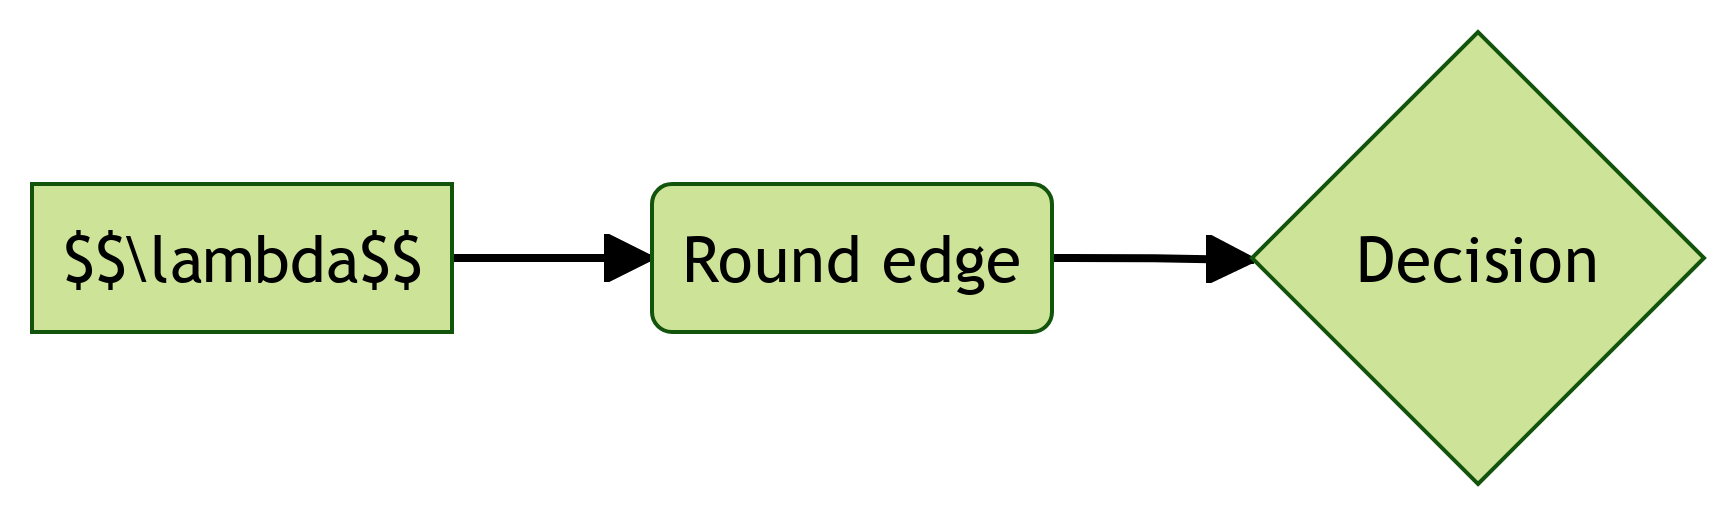
\includegraphics[width=5.5in,height=3.12in]{TCC_files/figure-latex/mermaid-figure-1.png}

}

\caption{\label{fig-arvore}Exemplo de estrutura de árvore de regressão.
A árvore tem cinco folhas e quatro nós internos.}

\end{figure}%

\vspace{12pt}

~~~Descrevendo formalmente o processo de construção de uma árvore de
regressão\footnote{Uma árvore de regressão é um caso específico da
  árvore de decisão, mas para regressão.}, a sua execução é composta por
dois passos. No primeiro passo, dividimos o espaço dos preditores em
\(J\) regiões distintas e disjuntas denotadas por
\(R_1, R_2, ..., R_J\). No segundo passo, para cada observação que
pertence a região \(R_j\), a previsão será a mesma. Essa previsão será
simplesmente a média dos valores da variável dependente das observações
de treinamento que estão dentro da região \(R_j\) (JAMES \emph{et al.},
2013). Dessa forma, dado que se tenha duas regiões \(R_1\) e \(R_2\), e
a média dos valores da variável resposta tenha sido 10 e 20,
respectivamente. Então, Para uma observação \(X = x, x \in R_1\), o
valor previsto será 10 e, caso contrário, se \(x \in R_2\), o valor
previsto será 20.

\vspace{12pt}

~~~As regiões \(R_1, R_2, ..., R_J\) são construídas em formato de caixa
de forma a minimizar a soma dos quadrados. Dessa forma, podemos modelar
a variável resposta como uma constante \(c_m\) em cada região \(R_j\).
Assim, definimos a resposta:

\[
f\left(x\right) = \sum^J_{j=1}c_j I\left(x \in R_j \right)
\]

\vspace{12pt}

~~~Agora, utilizando o critério de minimizar a soma dos quadrados,
deve-se minimizar
\(\sum_{x_i \in R_j} \left[y_i - f\left(xi\right)\right]^2\) para
encontrar um estimador para o parâmetro \(c_j\). No entanto, perceba que
\(f\left(x_i\right)\) está sendo avaliado somente em um ponto específico
\(x_i\), o que reduzirá \(f\left(x_i\right)\) para uma constante
\(c_j\). É fácil de se chegar ao resultado se observarmos a definição da
função indicadora \(I\left(x \in R_j \right)\):

\[
I_{R_j}(x_i) =
\begin{cases}
    1,& \text{se } x_i \in R_j \\
    0,& \text{se } x_i \notin R_j
\end{cases}
\] e, como um ponto \(x_i\) não pode estar ao mesmo tempo em duas
regiões \(R_j\), pois as regiões são disjuntas, temos que apenas um dos
casos a função indicadora será diferente de 0. Portanto,
\(f\left(x_i\right) = c_j\). Assim, derivando
\(\sum_{x_i \in R_j} \left(y_i - c_j\right)^2\) em relação a \(c_j\)

\begin{equation}\phantomsection\label{eq-partial}{
\frac{\partial{\sum_{x_i \in R_j} \left(y_i - c_j\right)^2}}{\partial{c_j}} = -2\sum_{x_i \in R_j} \left(y_i - c_j\right)
}\end{equation} e igualando Equação~\ref{eq-partial} a 0, temos a
seguinte equação \[
\sum_{x_i \in R_j} \left(y_i - \hat{c}_j\right) = 0
\] que se abrirmos o somatório e dividirmos pelo número total de pontos
\(N_{j}\) na região \(R_j\), teremos que o estimador de \(c_j\) será
somente a média dos \(y_i\) na região \(R_j\):

\begin{equation}\phantomsection\label{eq-estimacj}{
\sum_{x_i \in R_j} y_i - c_j \sum_{x_i \in R_j} 1 = 0 \Longrightarrow \hat{c}_j = \frac{1}{N_{j}}\sum_{x_i \in R_j} y_i
}\end{equation}

\vspace{12pt}

No entanto, JAMES \emph{et al.} (2013) caracteriza como inviável
considerar todas as possíveis partições do espaço das variáveis em \(J\)
caixas devido ao alto custo computacional. Dessa forma, a abordagem a
ser adotada é uma divisão binária recursiva. O processo começa no topo
da árvore de regressão, o ponto em que contém todas as observações, e
continua sucessivamente dividindo o espaço dos preditores. As divisões
são indicadas como dois novos ramos na árvore, como pode ser visto na
Figura~\ref{fig-arvore}.

\vspace{12pt}

Para executar a divisão binária recursiva, deve-se primeiramente
selecionar a variável independente \(X_j\) e o ponto de corte \(s\) tal
que a divisão do espaço dos preditores conduza a maior redução possível
na soma dos quadrados dos resíduos. Dessa forma, definimos dois
semi-planos

\[
R_{1}\left(j, s\right) = \{X | X_j \leq s\} \text{ e } R_{2}\left(j, s\right) = \{X | X_j > s\}
\] e procuramos a divisão da variável \(j\) e o ponto de corte \(s\) que
resolve a equação

\[
\min_{j, s}\left[\min_{c_1} \sum_{x_i \in R_1\left(j, s\right)} \left(y_i - c_{1}\right)^2 + \min_{c_2} \sum_{x_i \in R_2\left(j, s\right)} \left(y_i - c_{2}\right)^2\right]
\] em que \(c_1\) e \(c_2\) é a média da variável dependente para as
observações de treinamento nas regiões \(R_1\left(j, s\right)\) e
\(R_2\left(j, s\right)\), respectivamente. Assim, encontrando a melhor
divisão, os dados são particionados nas duas regiões resultantes e o
processo de divisão é repetido em todas as outras regiões.

\vspace{12pt}

~~~O tamanho da árvore pode ser considerado como um hiperparâmetro para
regular a complexidade do modelo pois, uma árvore muito grande pode
causar um ajuste excessivo aos dados de treinamento, capturando não
apenas os padrões relevantes, mas também os ruído. Dessa forma, o modelo
apresenta um bom desempenho nos dados de treinamento, mas não consegue
desempenhar bem em dados que não foram observados devido a sua
incapacidade de generalizar. Não obstante, uma árvore pequena pode não
capturar os padrões, relações e estruturas importantes contidas nos
dados. Dessa forma, adotamos como estratégia para selecionar o tamanho
da árvore é crescer uma grande árvore \(T_0\) e interromper o processo
de divisão apenas quando atingir um tamanho mínimo de nós. No fim, a
grande árvore \(T_0\) é podada usando o critério custo de complexidade,
que será definida a seguir.

\vspace{12pt}

~~~Para o processo de poda da árvore, definimos uma árvore qualquer
\(T\) que pode ser obtida através do processo de poda de \(T_0\) e
portanto \(T \subset T_0\). Dessa forma, sendo \(N_j\) a quantidade de
pontos na região \(R_j\), seja

\[
\begin{aligned}
\hat{c}_j &= \frac{1}{N_j}\sum_{xi \in R_j} y_i \\
Q_j\left(T\right) &= \frac{1}{N_j} \sum_{x_i \in R_j}\left(y_i - \hat{c}_j\right)^2
\end{aligned}
\] \(\hat{c}_j\) a média das observações da variável dependente na
\(R_j\) do nó interno \(j\) e \(Q_j\left(T\right)\) uma estatística
medidas de impureza do nó pelo erro quadrático. Assim, definimos o
critério custo de complexidade:

\[
C_{\alpha}\left(T\right) = \sum_{m = 1}^{|T|}N_jQ_j\left(T\right) + \alpha |T|
\] em que \(|T|\) denota a quantidade total de folhas e
\(\alpha \geq 0\) é o parâmetro de tunagem que equilibra o tamanho da
árvore e a adequação aos dados de forma que para cada \(\alpha\), a
árvore \(T_{\alpha} \subseteq T_0\) minimiza
\(C_{\alpha}\left(T\right)\). Valores grandes para \(\alpha\) resulta em
árvores menores, valores menores resulta em árvores maiores e
\(\alpha = 0\) resulta na própria árvore \(T_0\). A procura por
\(T_{\alpha}\) consiste em sucessivamente colapsar o nó interno que
produz o menor aumento em \(\sum_j N_j Q_j\left(T\right)\) e o processo
continua até produzir uma árvore de um único nó. Esse processo gera uma
sequência de subárvores que contém uma única menor subárvore que, para
cada \(\alpha\), minimiza \(C_{\alpha}\left(T\right)\). Além disso, a
estimação de \(\alpha\) é feita por validação cruzada com cinco ou dez
folds, e a estimativa \(\hat \alpha\) é escolhida para minimizar a soma
dos quadrados dos resíduos durante a validação cruzada. Assim, a árvore
final será \(T_{\hat \alpha}\). O  Algoritmo~\ref{algo-buildtree} 
exemplifica o processo de crescimento de uma árvore de regressão:

\begin{algo}

\centering{

\begin{algorithm}[H]
\caption{Algoritmo para crescer uma árvore de regressão}
\begin{algorithmic}
\State \textbf{1.} Use a divisão binária recursiva para crescer uma árvore grande $T_0$ nos dados de treinamento, parando apenas quando cada folha tiver menos do que um número mínimo de observações.

\vspace{3.7pt}

\State \textbf{2.} Aplique o critério custo de complexidade à árvore grande \( T_0 \) para obter uma sequência de melhores subárvores \( T_\alpha \), em função de \( \alpha \).

\vspace{3.7pt}

\State \textbf{3.} Use validação cruzada K-fold para escolher \( \alpha \). Isto é, divida as observações de treinamento em K folds. Para cada \( k = 1, \ldots, K \):
    \State \hspace{1em} (a) Repita os Passos 1 e 2 em todos os folds, exceto no k-ésimo fold dos dados de
    \State \hspace{1em} treinamento.
    \State \hspace{1em} (b) Avalie o erro quadrático médio de previsão nos dados no k-ésimo fold deixado
    \State \hspace{1em} de fora, em função de \( \alpha \). Faça a média dos resultados para cada valor de \( \alpha \) e
    \State \hspace{1em} escolha \( \alpha \) que minimize o erro médio.

\vspace{3.7pt}

\State \textbf{4.} Retorne a subárvore \( T_{\hat{\alpha}} \) do Passo 2 que corresponde ao valor estimado de \( \alpha \).
\end{algorithmic}
\end{algorithm}

}

\caption{\label{algo-buildtree}Fonte: JAMES \emph{et al.} (2013, p.
337).}

\end{algo}%

\section{Métodos Ensemble}\label{muxe9todos-ensemble}

~~~As árvores de decisão são conhecidas por sua alta interpretabilidade,
mas geralmente apresentam um desempenho preditivo preditivo inferior em
comparação com outros modelos e algoritmos. No entanto, é possível
superar essa limitação construindo um modelo preditivo que combina a
força de uma coleção de modelos base mais simples, um processo conhecido
como aprendizado Ensemble. De acordo com HASTIE \emph{et al.} (2009), o
aprendizado Ensemble pode ser dividido em duas etapas principais: a
primeira etapa consiste em desenvolver uma população de algoritmos de
aprendizado base a partir dos dados de treinamento, e a segunda etapa
envolve a combinação desses algoritmos para formar um estimador
agregado. Portanto, nesta seção, serão definidos os métodos de
aprendizagem Ensemble utilizados neste trabalho. O foco inicial será no
Random Forest, seguido pela descrição e explicação teórica do Bagging,
Boosting, Stacking e outros algoritmos de aprendizado de máquina.

\subsection{Bagging}\label{bagging}

~~~O algoritmo de Bootstrap Aggregation, ou Bagging, foi introduzido por
BREIMAN (1996). Sua ideia principal é gerar um estimador agregado a
partir de múltiplas versões de um preditor, que são formadas fazendo
réplicas bootstrap do conjunto de treinamento e utilizando-as como novos
conjuntos de treinamento. O Bagging pode ser utilizado como uma forma de
melhorar a estabilidade, precisão de modelos ou algoritmos de
aprendizado de máquina, além de diminuir a variância e evitar
sobreajuste. Por exemplo, o Bagging poderia ser utilizada para melhorar
a árvore de regressão que foi descrita anteriormente, mas também poderia
ser aplicado a outros métodos.

\vspace{12pt}

~~~BREIMAN (1996) define formalmente o algoritmo de Bagging, no qual
temos um conjunto de treinamento \(\mathcal{L}\). Tomamos amostras
bootstrap \(\mathcal{L}^{\left(B\right)}\) com \(B\) réplicas de
\(\mathcal{L}\) para formar
\(\{\varphi \left(x, \mathcal{L}^{\left(B\right)}\right)\}\), onde
\(\varphi\) denota um modelo ou algoritmo treinado nas amostras
bootstrap \(\{\mathcal{L}^{\left(B\right)}\}\) com variáveis
independentes \(x\) para previsão ou classificação de uma variável
dependente \(y\). Caso a variável dependente \(y\) seja numérica, a
predição é feita tomando a média de
\(\varphi \left(x, \mathcal{L}^{\left(B\right)}\right)\). Assim, temos
que a predição é feita da seguinte forma:

\[
\varphi_{B}\left(x\right) = \frac{1}{B} \sum_{b = 1}^B \varphi \left(x, \mathcal{L}^{\left(B\right)}\right)
\] onde \(\varphi_{B}\) denota a agregação. Não obstante, se \(y\)
prediz uma classe, utilizamos a votação majoritária. Ou seja, se
estivermos classificando classes \(j \in {1, \dots, J}\), então podemos
tomar
\(N_j = \#\{B; \varphi\left(x, \mathcal{L}^{\left(B\right)}\right) = j\}\)
que representa a quantidade de vezes que a classe \(j\) foi predita
pelos estimadores. Assim, tomamos \[
\varphi_{B}\left(x\right) = \arg \min_{j} N_j
\] isto é, o \(j\) para o qual \(N_j\) é máxima.

\vspace{12pt}

~~~Embora a técnica de Bagging tenha o poder de melhorar o desempenho de
uma árvore de regressão ou classificação, isso é alcançado ao custo de
menor interpretabilidade. No caso da aplicação de Bagging para uma
árvore de regressão, construímos \(B\) árvores de regressão usando \(B\)
réplicas de amostra bootstrap e tomamos a média das predições
resultantes (JAMES \emph{et al.}, 2013). Nesse caso, as árvores de
regressão crescem ao máximo, sem passar pelo processo de poda,
resultando em cada árvore individual com alta variância, mas baixo viés.
No entanto, ao agregarmos \(\varphi_{B}\) das \(B\) árvores, reduzimos a
variância. Para mitigar a falta de interpretabilidade do método Bagging
aplicado a uma árvore de regressão, podemos utilizar a soma do quadrado
dos resíduos como uma estatística da importância das variáveis
independentes. Um valor elevado da redução total média da soma do
quadrado dos resíduos devido às divisões em um determinado preditor,
calculada sobre todas as árvores \(B\), indica um preditor importante.

\subsection{Random Forest}\label{random-forest}

A Random Forest é uma técnica derivada do método de Bagging. No entanto,
a Random Forest providencia uma melhora fazendo um ajuste aleatório que
diminui a correlação entre as \(B\) árvores.

\subsection{Boosting}\label{boosting}

\subsection{Stacking}\label{stacking}

\subsection{Gradient Boosting}\label{gradient-boosting}

\subsection{Categorical Boosting}\label{categorical-boosting}

\subsection{Light Gradient-Boosting}\label{light-gradient-boosting}

\subsection{Extreme Gradient Boosting}\label{extreme-gradient-boosting}

\vspace{12pt}

\chapter{Metodologia}\label{metodologia}

\section{Os dados e o procedimento adotado para sua
obtenção}\label{os-dados-e-o-procedimento-adotado-para-sua-obtenuxe7uxe3o}

--- AINDA SERÁ MODIFICADO ---

~~~O Web scraping, também conhecido como extração de dados da web, é uma
técnica utilizada para o processo de coleta de dados estruturados da web
de maneira automatizada. É um processo que vem sendo constantemente
utilizado por instituições públicas e privadas para a construção de
produtos que utilizam algoritmos de aprendizagem de máquinas, observa
ofertas e discontos, faz análise de mercado ou monitoração de marcas.

\vspace{12pt}

Neste projeto, para fins de estudo e análise do mercado imobiliário, os
dados foram coletados por meio de extração de dados do site do Zap
Imóveis. O Zap Imóveis é um site do Grupo OLX que reúne ofertas do
mercado imobiliário e que funciona como uma plataforma dinâmica para
facilitar a conexão entre quem deseja alugar, comprar ou vender um
imóvel; podendo servir também para corretores ou outros profissionais do
setor de imóveis. Este projeto foi possível graças as informações que
foram coletadas do site do Zap Imóveis em dois diferentes períodos do
ano de 2023. O primeiro deles, as informações foram coletadas utilizando
variados pacotes para raspagem de dados e proxies rotativas da linguagem
de programação R, a fim de evitar ser bloqueado pelos mecanismos de
segurança do site. Na segunda etapa, os dados foram coletados empregando
a linguagem de programação Python com as bibliotecas Scrapy e Playwrite,
que serve para web crawling e web scraping, e o Playwrite que serve para
testes em aplicativos da web, mas que neste caso foi utilizado para
manejar páginas dinâmicas.

\vspace{12pt}

Desta forma, com a ideia de modelar o valor do imóvel e analisar o
mercado imobiliário, foram coletados aqueles variáveis que estavam
disponíveis no site do Zap Imóveis e que poderiam de alguma forma ser
significativas ao tentar explicar o valor do imóvel durante a sua
modelagem. Assim, no total foram coletatas 23 variáveis, das quais 8 são
quantitativas e 15 qualitativas nominais, sendo 13 de caráter
dicotômico. No entanto, nem todas essas variáveis foram coletadas
diretamente do Zap Imóveis, a latitude e longitude foram obtidas pela
geocodificação do endereço utilizando o pacote tidygeocoder da linguagem
de programação R. Portanto, temos as seguites variáveis:

\begin{itemize}
\item
  Valor do imóvel: esta é a variável dependente, aquela que será
  modelada e será o principal objeto de estudo deste trabalho;
\item
  Área: área do imóvel em \(m^2\);
\item
  Condomínio: valor pago pelo condomínio;
\item
  IPTU: imposto cobrado de quem tem um imóvel urbano;
\item
  Banheiro: quantidade de banheiros presentes na propriedade;
\item
  Vaga de estacionamento: quantidade total de vagas de estacionamento;
\item
  Quarto: quantidade de quartos no imóvel;
\item
  Latitude: posição horizontal medida em frações decimais de graus;
\item
  Longitude: posição vertical que, assim como a latitude, é medida em
  frações decimais de graus;
\item
  Tipo do imóvel: foram obtidos 7 tipos de imóveis, apartamentos, casas,
  casas comerciais, casas de condomínio, casas de vila, coberturas,
  lotes comerciais e de condomínio;
\item
  Endereço: nome do endereço do imóvel;
\item
  Variáveis dicotômicas que indicam se o imóvel tem ou não aquela
  característica (representado como 1 ou 0, respectivamente): área de
  serviço, academia, elevador, espaço gourmet, piscina, playground,
  portaria 24 horas, quadra de esporte, salão de festa, sauna, spa e
  varanda gourmet.
\end{itemize}

\vspace{12pt}

No entanto, devido a observações feitas durante o estudo, nem todas
essas variáveis foram utilizadas para a modelagem do valor dos imóveis,
seja por conter muitos valores valores ausentes ou por não ter se
mostrado significante para o que se desejava explicar. Ainda, como a
coleta destes dados foram feitas em dois momentos distintos, temos dois
bancos de dados, um com 29712 observações e o outro com 14956. Por fim,
essas duas bases de dados foram unidas e, para não correr o risco de
conter imóveis repetidos, aqueles que tinham o mesmo número de
identificação foram removidos.

\section{Descritiva dos dados}\label{descritiva-dos-dados}

~~~A análise exploratória de dados marca uma das primeiras etapas de
qualquer estudo que utiliza a estatística como uma de suas principais
ferramentas, pois permite encontrar padrões de comportamento no dados,
descobrir relações entre as variáveis estudadas. Dessa forma, a primeira
etapa desse estudo, após a coleta e organização dos dados obtidos do Zap
Imóveis, foi fazer uma descritiva dos dados. Essa etapa permitiu
encontrar padrões nos diferentes tipos de imóveis bem como o seu tipo
pode influenciar na características do imóvel, o que, por consequência,
pode afetar o seu valor. Assim, para identificar esses diferentes
comportamentos, foram criados gráficos e tabelas a fim de caracterizar
as relações das variáveis independentes com a dependente.

\section{Aprendizado Supervisionado e não
supervisionado}\label{aprendizado-supervisionado-e-nuxe3o-supervisionado}

~~~Na aprendizagem de máquinas, uma das estapas mais importantes é saber
qual técnica será utilizada para resolver um problema que se enquadra em
diferentes formas de aprendizado. Para isso, existem mais de uma forma
em que um algoritmo consegue utilizar os dados e explicar o que está
sendo modelado a partir deles. No entanto, a maioria dos problemas de
aprendizado de máquinas recais em dois casos mais conhecidos:
aprendizado supervisionado e não supervisionado.

\subsection{Aprendizado
supervisionado}\label{aprendizado-supervisionado}

~~~Suponha uma regressão logística. Sabemos que na regressão logistíca
temos um modelo com a seguinte forma
\(Y_i = f\left(X\right) + \epsilon\), em que \(Y_i\) assume 0 ou 1 para
classificar o que está sendo modelado e representa a variável
dependente, \(f\left(X\right)\) representa as variáveis independentes
que serão utilizadas para a modelagem e \(\epsilon\) representa o erro
da regressão. Dessa forma, podemos considerar o caso em que a regressão
logística tenta classificar pacientes que podem ou não estar com
diabetes. Para isso, utilizariamos variáveis significativas para a
classificação do estado de cada paciente. Esse exemplo é conhecido como
aprendizagem supervisionada. Na aprendizagem supervisionada, busca-se
aprender \(Y_i\) atráves de um exemplo. Nesse caso, as variáveis
dependentes podem ser interpretadas como o exemplo, as informações de
relações de pacientes que podem ter ou não diabetes, e o estado do
paciente pode ser interpretado como o que se deseja aprender. Este
processo é entendido como \emph{aprendizado por exemplo}, HASTIE
\emph{et al.} (2009). O aprendizado supervisionado pode aparecer em
casos de regressão linear, regressão logística, ou até mesmo em métodos
mais modernos, como GAM, boosting e máquina de vetores de suporte, JAMES
\emph{et al.} (2013).

\subsection{Aprendizado não
supervisionado}\label{aprendizado-nuxe3o-supervisionado}

~~~Por outro lado, o aprendizado não supervisionado aparece em situações
mais desafiadores, pois não há um exemplo para explicar aquilo que se
pretende explicar. Este processo é conhecido como \emph{aprendizado sem
exemplo}, HASTIE \emph{et al.} (2009). Dessa forma, no aprendizado não
supervisionado, tem-se uma amostra com N observações
\(\left(x_1, ..., x_N\right)\) de um vetor aleatório \(X\) com densidade
conjunta \(f\left(x\right)\) em que o objetivo é inferir propriedades da
densidade sem ajuda de exemplos para cada observação. Assim, como há uma
falta de uma variável resposta \(y_i\) para supervisionar a análise,
pode-se procurar entender a relação entre as variáveis ou as
observações, JAMES \emph{et al.} (2013). Por exemplo, uma das técnicas
mais aplicadas em problemas que envolvem o aprendizado supervisionado é
a análise de cluster, em que o objetivo é determinar, com base em
\(x_1, ..., x_n\), se as observações são caracterizadas em grupos
distintos. Esse é um dos métodos que poderiam ser aplicados, por
exemplo, na análise de crédito de clientes de um cartão de crédito,
tornando possível analisar o seu perfil e classificá-lo em diferentes
grupos para recomendar produtos especificos adequados ao seu perfil.

\section{Reamostragem para avaliação de
performance}\label{reamostragem-para-avaliauxe7uxe3o-de-performance}

~~\\

~~\\

\section{Métricas de avaliação}\label{muxe9tricas-de-avaliauxe7uxe3o}

~~\\

\section{Tunagem de
hiperparâmetros}\label{tunagem-de-hiperparuxe2metros}

~~~Na aprendizagem de máquina, uma das etapas fundamentais é a tunagem
dos hiperparâmetros dos algoritmos de aprendizagem. Essa etapa consiste
em encontrar a melhor combinação de hiperparâmetros e, consequentemente,
resultando em uma configuração algoritmo que proporciona melhor
performance e capacidade de generalização. No entanto, essa configuração
não é trivial.

\vspace{12pt}

~~~Os algoritmos de otimização de hiperparâmetros procuram pelo melhor
ajuste de hiperparâmetros \(\lambda \in \tilde{\Lambda}\) para um
algoritmo de aprendizagem \(I_{\lambda}\). O espaço de procura
\(\tilde{\Lambda} \in \Lambda\) contém todas as possíveis configurações
de hiperparâmetros consideradas para otimização. Dessa forma, temos que:

\begin{equation}\phantomsection\label{eq-space}{
\tilde{\Lambda} = \tilde \Lambda_1 \cup \tilde \Lambda_2 \cup ... \cup \tilde \Lambda_l
}\end{equation} em que \(l\) são todas as possíveis configurações de
hiperparâmetros. Além disso,
\(\tilde \Lambda_i \ \left(i = 1, 2, ..., l\right)\) representam o
subconjunto de limites dos domínios do i-ésimo hiperparâmetro
\(\Lambda_i\), podendo ser contínuo, discreto ou categórico (BISCHL et
al., 2023).

\vspace{12pt}

A busca pela melhor combinação de hiperparâmetros \(\lambda\) é feito de
forma iterativa, utilizando métodos de reamostragem para dividir o
conjunto de dados entre teste e treinamento. Portanto, para validar e
encontrar os hiperparâmetos, o algoritmo de aprendizagem é validado
através da divisão do conjunto de dados. Assim, tem-se a seguinte
estratégia de separação do conjunto de dados:

\begin{equation}\phantomsection\label{eq-teste}{
\mathcal{J} = \left(\left(J_{treino, 1},\ J_{teste, 1}\right), ..., \left(J_{treino, B},\ J_{test, B}\right)\right)
}\end{equation} onde \(J_{treino, i}, \ J_{teste, i}\) representam os
vetores de índices \(\left(i = 1, \, 2, ..., \ B\right)\) para os
conjuntos de treino e teste, respectivamente, e \(B\) representa o
número total de divisões.

\vspace{12pt}

A motivação para fazer a divisão do conjunto de dados entre treino e
teste é ajustar o algoritmo em dados reais e avaliar a sua performance
em dados ainda não vistos, processo representado pelo banco de treino e
teste, respectivamente. Para fazer a avaliação dessa performance é
necessário estimar uma métrica de performance em cada divisão. Assim,
para um dado algoritmo \(I_{\lambda}\) é calculado uma métrica de
performance \(\rho\) para cada \(J_{teste, i}\) após o ajuste do
algoritmo no \(J_{treino, i}\). Por fim, pode ser calculado uma média
amostral da métrica de cada uma das divisões. Dessa forma, o problema de
otimizar os hiperparâmetros pode ser definida da seguinte forma:

\[
\lambda^* \in \underset{\lambda \in \tilde \Lambda}{\operatorname{argmin}} \ c\left(\lambda \right)
\] onde \(\lambda^*\) denota a melhor combinação possível de
hiperparâmetros, \(c\left(\lambda \right)\) representa a generalização
do erro, podendo ser representado também por
\(\widehat{GE}\left(I, \ \mathcal J, \ \rho, \ \lambda\right)\), quando
\(I, \ \mathcal{J}, \ \rho\) são fixados e \(I\) denota um algoritmo de
aprendizagem de máquina. O erro de generalização é estimado e otimizado
a fim de evitar um ajuste excessivo (overfitting), podendo prejudicar
quando o algoritmo fizer estimativas em dados ainda não vistos. Assim, o
processo pode ser visualizado pela figura Figura~\ref{fig-hpo}:

\begin{figure}

\centering{

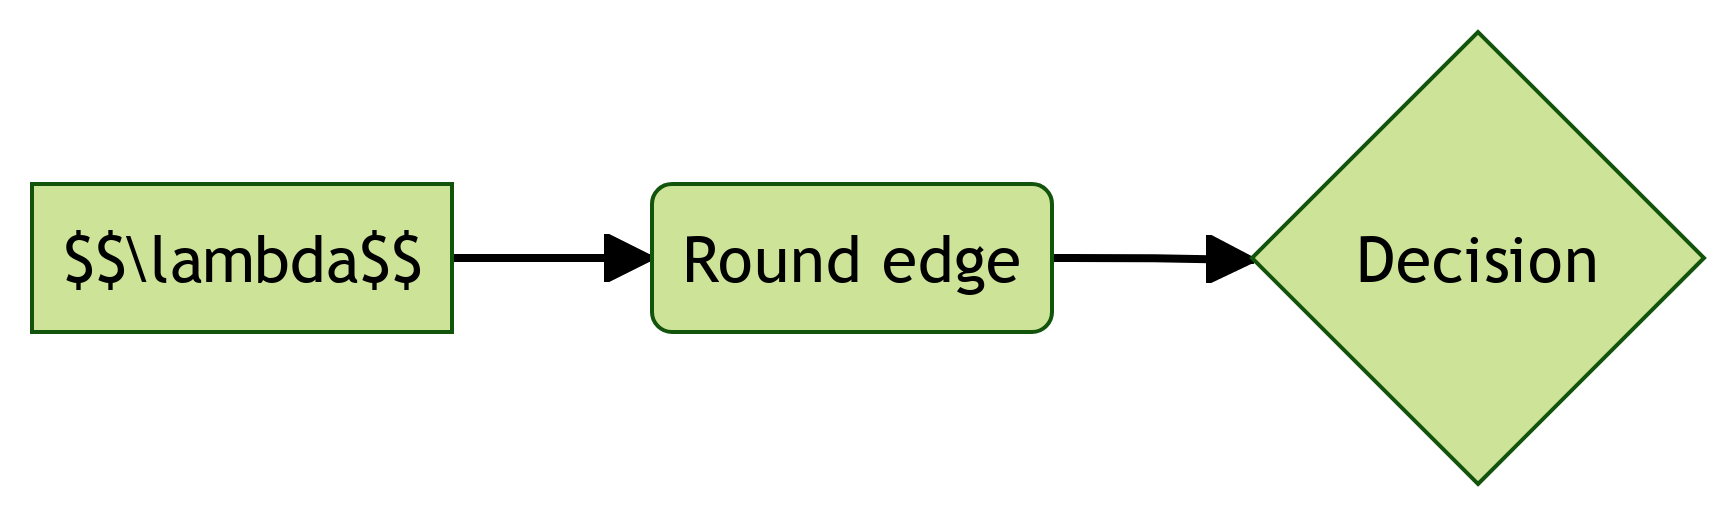
\includegraphics[width=4.5in,height=1.3in]{TCC_files/figure-latex/mermaid-figure-2.png}

}

\caption{\label{fig-hpo}Processo de otimização de hiperparâmetros}

\end{figure}%

\vspace{12pt}

\subsection{Otimização Bayesiana}\label{otimizauxe7uxe3o-bayesiana}

~~~Existem diversas técnicas para otimização de hiperparâmetros
utilizadas em aprendizagem de máquina. Uma das técnicas mais comuns é o
GridSearch. BISCHL \emph{et al.} (2023) definem GridSearch como um
processo que divide o intervalo contínuo de valores possíveis de cada
hiperparâmetro em um conjunto de valores específicos e avalia
exaustivamente o algoritmo para todas as combinações possíveis. No
entanto, como todas as combinações possíveis aumentam exponencialmente
com a quantidade necessária para avaliação do algoritmo, o GridSearh tem
um custo computacional bastante elevado. Assim, existem algoritmos de
otimização mais sofisticados que entregam melhores performances, como a
otimização bayesiana, que foi utilizada neste trabalho.

\vspace{12pt}

~~~A otimização bayesiana não se refere a um tipo específico de
algoritmo de otimização, mas sim a uma filosofia de otimização baseada
em inferência bayesiana, a qual contém uma extensa família de algoritmos
de otimização (GARNETT, 2023). Não obstante, a otimização bayesiana tem
obtido benchmarks melhores que outros algoritmos em inúmeros problemas
complexos de otimização de hiperparâmetros (SNOEK; LAROCHELLE; ADAMS,
2012).

\vspace{12pt}

~~~Diferente de outros algoritmos de otimização de hiperparâmetros, a
otimização bayesiana determina as futuras tentativas de avaliação com
base em resultados obtidos previamente (YANG; SHAMI, 2020). Para a
definição dos pontos futuros, é utilizada uma função probabilística
\(P\left(\rho |  \lambda \right)\) (BERGSTRA; YAMINS; COX, 2013). Assim,
após o ajuste da função probabilística, tem-se como resultado para cada
\(\lambda\) uma estimativa da performance
\(\hat c \left(\lambda \right)\) e da predição da incerteza
\(\hat \sigma \left(\lambda \right)\), além de obter também a
distribuição preditiva da função probabilística. Com a distribuição
obtida, uma função de aquisição determina o trade-off entre exploitation
e exploration\footnote{exploitation pode ser entendido como procurar
  próximo a boas observações e}. Dessa forma, os algoritmos de
otimização bayesiana são definidos segundo a lei
\(\lambda \to c\left(\lambda \right)\) e procuram um equilíbrio entre o
processo de exploitation-exploration para detectar as regiões ótimas
mais prováveis e não perder melhores configurações em áreas ainda não
exploradas.

\subsection{Tree-Structured Parzen
Estimator}\label{tree-structured-parzen-estimator}

~~~Existem diversas funções probabilísticas para uso na otimização
bayesiana, algumas delas é o Processo Gaussiano, Random Forest ou
Tree-Structured Parzen Estimator (TPE). Nesse trabalho, foi utilizado o
Tree-Structured Parzen Estimator, utilizando a biblioteca Optuna (AKIBA
\emph{et al.}, 2019) para sua aplicação.

\vspace{12pt}

~~~O TPE define duas funções,
\(l\left(x\right) \text{ e } g\left(x\right)\), que são usadas para
modelar a distribuição das variáveis do domínio (YANG; SHAMI, 2020).
Utilizando as duas densidades, o TPE procura modelar a probabilidade de
se observar um hiperparâmetro \(x\) dado uma métrica de performance
\(\rho\). Dessa forma, tem-se a seguinte definição:

\begin{equation}\phantomsection\label{eq-tpe}{
p(x|y) =
\begin{cases}
    l(x) & \text{if } y < y^* \\
    g(x) & \text{if } y \ge y^*
\end{cases}
}\end{equation} em que \(l\left(x\right)\) é definido como a densidade
em que a função perda é menor que um limiar \(y^*\) e
\(g\left(x\right)\) representa é a densidade em que a função
perda\footnote{definição de função perda} tem valores acima do limiar
\(y^*\) (BERGSTRA \emph{et al.}, 2011). O limite \(y^*\) é escolhido
através de um hiperparâmetro \(\gamma\), onde \(\gamma\) representa o
percentil dos valores observados de \(y\), de modo que
\(p\left(y < y^*\right) = \gamma\).

\vspace{12pt}

Por padrão, o tree-structured parzen estimator tem como função de
aquisição o Expected Improvement \(\left(EI\right)\), que pode ser
otimizado para o TPE da seguinte forma:

\begin{equation}\phantomsection\label{eq-exp}{
  EI_{y^*}\left(x\right) = \int_{-\infty}^{y^*} \left(y^* - y\right)p\left(y | x\right) dy
}\end{equation}

Ainda, para encontrar a probabilidade marginal de \(x\), temos a
seguinte integral
\(p\left(x\right) = \int_{\mathbb{R}} p\left(x | y\right)p\left(y\right)dy\).
Particionando o domínio de \(y\), chega-se em:

\[
p\left(x\right) = \int_{-\infty}^{y^*} p\left(x | y\right)p\left(y\right)dy + \int_{y^*}^{\infty} p\left(x | y\right)p\left(y\right)dy = \gamma l\left(x\right) + \left(1 - \gamma \right) g\left(x\right)
\]

Assim, utilizando o Teorema de Bayes e fazendo as substituições na
integral da Equação~\ref{eq-exp}:

\[
EI_{y^*}\left(x\right) = \int_{-\infty}^{y^*} \left(y^* - y\right) \frac{p\left(x | y\right)p\left(y\right)}{p\left(x\right)}dy = \left(\gamma y^*  - \int_{-\infty}^{y^*} p\left(y\right)dy\right) \left(\gamma + \left(1 - \gamma\right)\frac{g\left(x\right)}{l\left(x\right)}\right) ^{-1}
\] em que a segunda expressão do produto mostra que para maximizar o
Expected Improvement é necessário pontos de \(x\) com maior
probabilidade em \(l\left(x\right)\) e com baixa probabilidade em
\(g\left(x\right)\). Não obstante, no TPE, maximizar o \(EI\) é
equivalente a maximizar a razão entre as duas distribuições
\(r\left(x\right) = \frac{l\left(x\right)}{g\left(x\right)}\)
(COWEN-RIVERS \emph{et al.}, 2022).

\newpage

\chapter{Capítulo 4}\label{capuxedtulo-4}

\section{Resultados}\label{resultados}

\newpage

\chapter{Conclusão}\label{conclusuxe3o}

\chapter{Referências}\label{referuxeancias}

\phantomsection\label{refs}
\begin{CSLReferences}{0}{1}
\bibitem[\citeproctext]{ref-optuna_2019}
AKIBA, T. \emph{et al.} Optuna: A Next-generation Hyperparameter
Optimization Framework. {[}S.l.{]}: {[}s.n.{]}, 2019.

\bibitem[\citeproctext]{ref-bergstra2011algorithms}
BERGSTRA, J. \emph{et al.} Algorithms for hyper-parameter optimization.
\textbf{Advances in neural information processing systems}, 2011. v. 24.

\bibitem[\citeproctext]{ref-bergstra2013making}
\_\_\_\_\_\_; YAMINS, D.; COX, D. Making a science of model search:
Hyperparameter optimization in hundreds of dimensions for vision
architectures. {[}S.l.{]}: PMLR, 2013. p. 115--123.

\bibitem[\citeproctext]{ref-bischl2023hyperparameter}
BISCHL, B. \emph{et al.} Hyperparameter optimization: Foundations,
algorithms, best practices, and open challenges. \textbf{Wiley
Interdisciplinary Reviews: Data Mining and Knowledge Discovery}, 2023.
v. 13, n. 2, p. e1484.

\bibitem[\citeproctext]{ref-breiman1996bagging}
BREIMAN, L. Bagging predictors. \textbf{Machine learning}, 1996. v. 24,
p. 123--140.

\bibitem[\citeproctext]{ref-cowen2022hebo}
COWEN-RIVERS, A. I. \emph{et al.} Hebo: Pushing the limits of
sample-efficient hyper-parameter optimisation. \textbf{Journal of
Artificial Intelligence Research}, 2022. v. 74, p. 1269--1349.

\bibitem[\citeproctext]{ref-garnett2023bayesian}
GARNETT, R. \textbf{Bayesian optimization}. {[}S.l.{]}: Cambridge
University Press, 2023.

\bibitem[\citeproctext]{ref-hastie2009elements}
HASTIE, T. \emph{et al.} \textbf{The elements of statistical learning:
data mining, inference, and prediction}. {[}S.l.{]}: Springer, 2009. V.
2.

\bibitem[\citeproctext]{ref-izbicki2020aprendizado}
IZBICKI, R.; SANTOS, T. M. Dos. \textbf{Aprendizado de m{á}quina: uma
abordagem estat{ı́}stica}. {[}S.l.{]}: Rafael Izbicki, 2020.

\bibitem[\citeproctext]{ref-james2013introduction}
JAMES, G. \emph{et al.} \textbf{An introduction to statistical
learning}. {[}S.l.{]}: Springer, 2013. V. 112.

\bibitem[\citeproctext]{ref-snoek2012practical}
SNOEK, J.; LAROCHELLE, H.; ADAMS, R. P. Practical bayesian optimization
of machine learning algorithms. \textbf{Advances in neural information
processing systems}, 2012. v. 25.

\bibitem[\citeproctext]{ref-yang2020hyperparameter}
YANG, L.; SHAMI, A. On hyperparameter optimization of machine learning
algorithms: Theory and practice. \textbf{Neurocomputing}, 2020. v. 415,
p. 295--316.

\end{CSLReferences}



\end{document}
